\documentclass[9pt,twocolumn,twoside]{pnas-report}

\usepackage{todonotes}

\setuptodonotes{inline,size=\small,color=blue!40}

\templatetype{pnasresearcharticle}

\usepackage{lipsum}


% set figures directory to be ./figures
\graphicspath{{./figures/}}

\title{\textcolor{red}{Draft} Security Analysis of Open-Source Software Package Ecosystems}

\author[a]{Žiga Trček}
\author[a]{Matej Urbas}
\author[a]{Jan Vasiljević}

\affil[a]{University of Ljubljana, Faculty of Computer and Information Science, Ve\v{c}na pot 113, SI-1000 Ljubljana, Slovenia}

\leadauthor{Jan Vasiljević}

\authordeclaration{All authors contributed equally to this work.}
\correspondingauthor{\textsuperscript{1}To whom correspondence should be addressed. E-mail: fine.author@email.com.}

\begin{abstract}
The use of open-source packages and libraries significantly accelerates software development but simultaneously introduces numerous security risks.
Motivated by a recent near-compromise of OpenSSH by a malicious actor, this study aims to investigate the security of open-source software by conceptualizing it as a network and examining transitive vulnerabilities.
Our analysis specifically focuses on PyPI, npm, and crates.io, which are the predominant package managers for Python, JavaScript, and Rust, respectively.
Through this exploration, we seek to uncover potential security weaknesses within these ecosystems and propose methods to enhance their security posture.

\todo{Ni se koncano: Cakam da mamo dejansk neki narejeno. Bolj placeholder.}
\end{abstract}
	
\dates{The manuscript was compiled on \today}
\doi{\href{https://ucilnica.fri.uni-lj.si/course/view.php?id=183}{Introduction to Network Analysis} 2023/24}

\begin{document}

\maketitle
\thispagestyle{firststyle}
\ifthenelse{\boolean{shortarticle}}{\ifthenelse{\boolean{singlecolumn}}{\abscontentformatted}{\abscontent}}{}

\dropcap{T}he date is March 28, 2024. A principal software engineer at Microsoft notices an unusual delay in his login attempts, timing at approximately 500ms—significantly longer than usual by his standards. This prompts an investigation into higher than normal CPU usage, during which he observes anomalous behavior in the SSH daemon process. This unexpected discovery leads to the identification of a vulnerability in the XZ Utils library utilized by OpenSSH. The breach, orchestrated by a malicious actor through a combination of social engineering, code injection, and obfuscation, was set into motion over several years. Interestingly, the core code of OpenSSH remained untouched; instead, a transitive dependency was exploited. Had this vulnerability remained undetected, it could have potentially compromised a vast number of servers relying on OpenSSH, embedding a remote code execution backdoor.


In a manner similar to the exploitation of the XZ Utils library, other open-source software packages and libraries are also vulnerable to malicious attacks.
The development of software inherently involves placing trust in the authors of utilized libraries, who are often individual hobbyists or small teams with limited resources.
The potential for significant damage is large if a malicious actor targets a lesser-maintained package that, while small, is widely used—either directly or as a transitive dependency in other software projects.
The incident involving the left-pad package, which was removed from npm and consequently led to the failure of numerous dependent packages, serves as a reminder of the inherent fragility within the open-source ecosystem.

Int this project we look at three different pacakge ecosystems: PyPI, npm, and crates.io, which are package repositories for Python, JavaScript, and Rust, respectively. We aim to investigate the security of these ecosystems by conceptualizing them as networks.... \textcolor{red}{Zej ne bom pisal dokler ne dejansko necesa nardimo.}

\begin{figure}
	\centering
	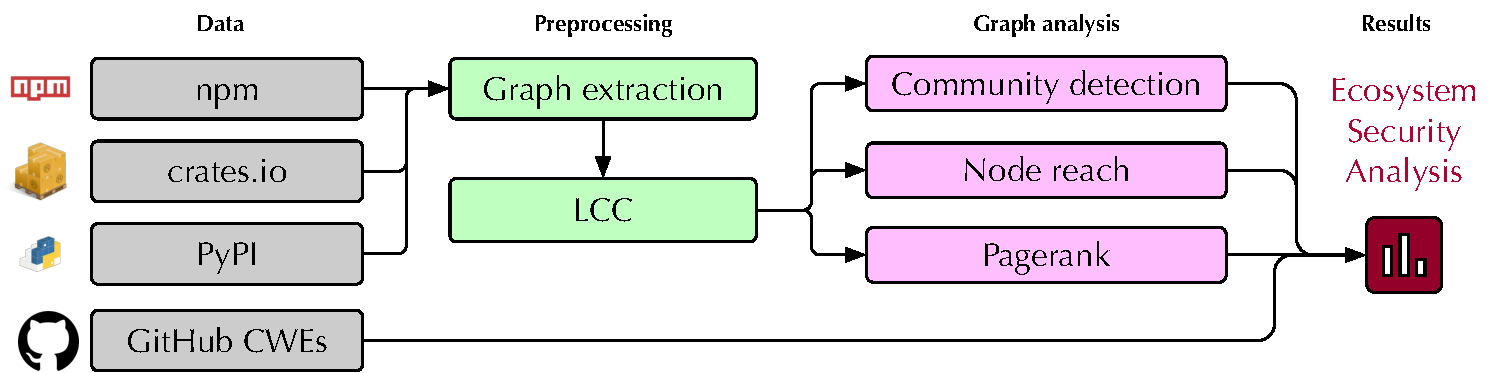
\includegraphics[width=1\linewidth]{topdown.pdf}
	\caption{Mandatory informative illustration highlighting main contributions.}
	\label{fig:topdown}
\end{figure}

\todo{Problem definition,  contributions etc. }


\section*{Related work}

Robustness of dependency networks is a topic that has been examined in several studies.
\cite{hafner2021robustness} explored the robustness of the npm package dependency network and highlighted its vulnerability to targeted attacks by identifying crucial nodes.
Attacks on such nodes could gravely affect a large portion of the network, as they are responsible for a significant number of dependencies.
Their findings suggest that while the network has crucial nodes, it is not highly vulnerable as they are mostly large and well-maintained projects.
Moreover, the network is trending towards a more robust state, as the number of dependencies is decreasing over time.

\cite{decan2018evolution} published a comparative analysis of dependency networks across 7 package ecosystems, including Cargo, CPAN, CRAN, npm, NuGet, Packagist, and RubyGems.
They proposed metrics to capture growth, changeability, reusability, and fragility.
They revealed that while the ecosystems are growing, a minority of packages are responsible for most updates and dependencies.
Furthermore, it is suggested that even transitive dependencies on unmaintained or obsolete packages can have a detrimental effect on the security and maintainability of the ecosystem.

\cite{tsakpinis2024accessibility} carried out a study on the accessibility of GitHub repositories for npm and PyPI libraries to understand the level of maintenance for them.
Their research showed that a significant portion of libraries lacked valid repository URLs, which hinders the ability to monitor vulnerabilities and maintain codebases.
An emphasis on the importance of maintaining valid repository URLs was made, as it is crucial for the sustainability of the open-source ecosystem.

Community detection has been proposed as a security analysis tool.
The found communities can provide great insight into the structure of the network and the relationships between packages, which helps assess the robustness of the network.
Understanding what packages are closely related and how they are connected can help identify potential vulnerabilities and dependencies that could be exploited by attackers \cite{hafner2021robustness, tsakpinis2024accessibility}.

\cite{korkmazrpackages} examine the dependency graph of R packages and the relationship between various metrics.
They find that centrality measures have a high correlation with the number of downloads and citations of a package.
Furthermore, package attributes such as number of authors and commits also have a positive impact on the number of downloads and citations.

Security vulnerability data analysis has been a large area of research in the recent years.
\cite{decan2018vulnerabilities} studied around 400 security reports from the npm network to understand how they are discovered and fixed, and how they affect the network.
They found that it takes around a year for a discovered vulnerability to be published publically, while it takes around 2 years after the discovery for the vulnerability to be fixed.
\cite{shahzad2012} study vulnerability life cycles on a large software vulnerability dataset, getting similar results.

\cite{HANIF2021103009} propose and evaluate novel machine learning approaches to vulnerability prediction in open-source software.
Some simple vulnerabilities are easily detected by their approach, but even more complex vulnerabilities can be detected with high accuracy.

\cite{hejderup2018} use call graphs instead of dependency graphs to detect dependencies in software.
They find that call graphs are efficient in aiding preliminary evaluation of security issues and their impact to other applications.
Furthermore, \cite{hejderup2022prazi} find that Cargo packages call only 40\% of their dependencies, which can lead to many unneeded security vulnerabilities.

\cite{ruohonen2021} examine around 200000 PyPI packages using static analysis and find that around 46\% of the packages have at least one security vulnerability.

\section*{Results}
We analysed three popular programming languages' ecosystems: npm \cite{NPM}, Crates.io \cite{crates} and PyPI \cite{pypi}.
Basic stats of each ecosystem's dependency network are shown in Table \ref{tab:basic_stats}.
NPM dependency network is analysed twice, once with combined production and development dependencies, and once with only production dependencies.

\begin{table}[h]\centering%
	\caption{Original dependency networks for all three ecosystems.}
	\begin{tabular}{l|ccccc}
		ecosystem  & $n$       & $m$        & $\langle k\rangle$ & $\langle C\rangle$ & \#CC     \\\hline
		npm        & $2425767$ & $23006281$ & $19$               & $0.18$             & $561569$ \\
		npm (prod) & $2424918$ & $7920337$  & $7$                & $0.06$             & $870151$ \\
		PyPI       & $532386$  & $1649201$  & $6$                & $0.11$             & $179304$ \\
		Crates.io  & $145269$  & $830337$   & $11$               & $0.23$             & $25179$  \\
	\end{tabular}
	\label{tab:basic_stats}
\end{table}

For the rest of our analysis, we only considered the largest weakly connected components.
Statistics of these networks are shown in Table \ref{tab:lcc_stats}.

\begin{table}[h]\centering%
	\caption{Largest connected components for all three ecosystems.}
	\begin{tabular}{l|ccccc}
		ecosystem  & $n$       & $m$        & $\langle k\rangle$ & $\langle C\rangle$ & \% nodes \\\hline
		npm        & $1845838$ & $22979692$ & $24$               & $0.23$             & $76$     \\
		npm (prod) & $1518107$ & $7871828$  & $10$               & $0.10$             & $62$     \\
		PyPI       & $349793$  & $1645588$  & $9$                & $0.17$             & $66$     \\
		Crates.io  & $119461$  & $829615$   & $13$               & $0.28$             & $82$     \\
	\end{tabular}
	\label{tab:lcc_stats}
\end{table}

By enumerating over vulnerabilities from the GitHub's advisory database we examined the reach of every listed vulnerability.
The vulnerabilities were analysed as if they all occured on the most recent package dependency graphs as we didn't have the required graph history snapshots.
The reach is defined by the size of the affected package's in-component - all the packages that directly or indirectly depend on the affected package.
To get a measure, which is proportional to the graph size and package importance, we summed up the page rank scores from the affected component.
The reach measure for every vulnerability for these ecosystems is shown in Figure \ref{fig:reach}.

\begin{figure}[t]\centering%
	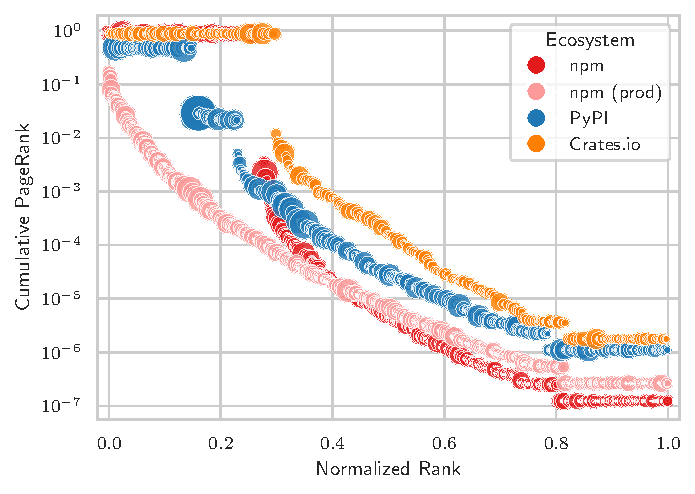
\includegraphics[width=\linewidth]{vuln_pagerank}
	\caption{Vulnerabilities and their reach. Each dot represents a single vulnerability. Dot size represents the vulnerability severity according to CVSS.  }
	\label{fig:reach}
\end{figure}

Crates.io and npm ecosystems are the most vulnerable.
Around 30\% of all vulnerabilities could reach almost every package (~95\% of all).
PyPI is a bit less interwined, with \textit{only} 69\% of packages being affected by the largest vulnerability.
If we exclude all development dependencies from the npm network, we notice a very high decrease in the percentage of affeceted packages.
The npm production network consists of around 3 times less edges than the network which also includes development dependencies.
This might correlate to 3 times the reduction in affected packages.
This also shows that developers are much more exposed than production environemtns, which keep their dependencies to the minimum.
Vulnerabilities with biggest reach for every ecosystem are listed in Table \ref{tab:highest_reach}.

\begin{table}[h]\centering%
	\caption{Biggest reach vulnerability.}
	\begin{tabular}{l|ccc}
		ecosystem  & package   & \% packages affected & affected pagerant \\\hline
		npm        & lodash    & $93$                 & $0.88$            \\
		npm (prod) & ms        & $\mathbf{30}$        & $\mathbf{0.18}$   \\
		PyPI       & pyOpenSSL & $69$                 & $0.54$            \\
		Crates.io  & shlex     & $95$                 & $0.88$            \\
	\end{tabular}
	\label{tab:highest_reach}
\end{table}

\section*{Discussion}

 {\bf Summary of results, main contributions, final conclusions, future work etc.}
\lipsum[1-3]

\small

\section*{Methods}

\todo{Verjetno manjka se ki}

\subsubsection*{Data Acquisition} The data for \texttt{crates.io} was acquired from their official website, where daily data dumps are available.
For \texttt{npm}, we initially attempted to follow the official guide on their website to clone the CouchDB database.
However, this method proved to be outdated and non-functional.
Consequently, we utilized data from \cite{npmdata}, which provides a weekly data dump of all npm dependencies.
The entire dataset was 200GB in size and packaged in a PostgreSQL database.
For \texttt{PyPI}, we had to manually scrape the data, as there is no official data dump available.

\subsection*{Data Preprocessing} From the data we acquired, we extracted package names, dependencies, and download counts. We then constructed a simple directed graph where nodes represent packages and edges represent dependencies. The edge direction is from the dependent package to the dependency. Graphs were then reduced to the largest connected component and exported in the \texttt{GraphML} format for further analysis.

\subsection*{\texttt{igraph}} Instead of relying on \texttt{networkx} for network analysis, we used the \texttt{igraph} library. Using \texttt{networkx}, even a simple import of the \texttt{npm} dataset took around 300 seconds. Additionally, every other operation was significantly slower compared to \texttt{igraph}.

\subsection*{Community Detection} For community detection, we used the \texttt{leiden} algorithm, which is an efficient method for uncovering community structures in large networks.
The algorithm optimizes the modularity function $ Q $ as $
	Q = \frac{1}{2m} \sum_{ij} \left[ A_{ij} - \frac{k_i k_j}{2m} \right] \delta(c_i, c_j)
$
where \( A_{ij} \) is the weight of the edge between nodes \( i \) and \( j \), \( k_i \) and \( k_j \) are the degrees of nodes \( i \) and \( j \), \( m \) is the total weight of all edges in the graph, and \( \delta(c_i, c_j) \) is the Kronecker delta which is 1 if nodes \( i \) and \( j \) belong to the same community and 0 otherwise.

\subsection*{Vulnerability analysis}

\normalsize

% \acknow{The authors would like to\dots}

% \showacknow{}

\bibliography{bibliography}

\end{document}
